
%packages a utilizar:
\documentclass{report}
\usepackage[T1]{fontenc}     % Fontes T1
\usepackage[utf8]{inputenc}  % Input UTF8
\usepackage[top=3cm,bottom=3cm,left=3cm,right=2.5cm,asymmetric]{geometry} %fronteiras
%\usepackage[nottoc]{tocbibind}
\usepackage[table]{xcolor} %Colorir tabelas
\usepackage[backend=biber, style=ieee]{biblatex} %bibliografia
\usepackage{csquotes}  % referências
\usepackage[portuguese]{babel} %Usar língua portuguesa
\usepackage{blindtext} 
\usepackage[printonlyused]{acronym}  %Acrónimos
\usepackage{hyperref}  %Autoref no índice
\usepackage{graphicx}  %Usar imagens
\usepackage{titling}
\usepackage{multicol} %multicoluna de texto
\usepackage{adjustbox}
\renewcommand{\figurename}{Fig.} 
\renewcommand{\tablename}{Tabela} 
\usepackage[font=small,tableposition=top]{caption} 
\usepackage[font=small]{subcaption}
\usepackage{xcolor} %cor nos textos
\usepackage{amsmath} %matematica
\usepackage{amssymb} %simbolos matematicos
\graphicspath{ {./images/} } %directorio das imagens
\usepackage{fancyhdr}
\usepackage{authblk}
\usepackage{float} %Posicionamento exacto das figuras no texto
\usepackage{url}   %referencias URL
\usepackage{blindtext}
\def\UrlBreaks{\do\/\do-} %não cortar referencias

\usepackage{indentfirst} %Garantir avanço do primeiro parágrafo
\hypersetup{pdfborder=0 0 0} %Remover a caixa vermelha das referências
\usepackage{chngcntr} %Numeração contínua das figuras
\counterwithout{figure}{chapter} %Numeração contínua de figuras
\counterwithout{table}{chapter} %Numeração contínnua de tabelas
\setlength{\parskip}{0.2cm} %Aumento de espaçamento entre parágrafos

\usepackage{hyperref}

 
\begin{document}	
	%Definições do Relatório

%Dados Gerais:
\def\titulo{Projecto Final: \\ Máquina de Lavagem de Roupa}
\def\data{Junho de 2022}
\def\versao{Ver.: 1.13}
\def\departamento{Departamento de Electrónica Telecomunicações e Informática}
\def\empresa{Universidade de Aveiro}
\def\logotipo{logotipo_ua.png}

%Dados dos Autores:
%primeiro autor:
\def\pautor{João Pedro Nunes Vieira} 
\def\numpautor{Nº Mec.:  50458}
\def\contactopautor{joaopvieira@ua.pt}
%segundo autor:
\def\sautor{Leandro Roque Costa} 
\def\numsautor{Nº Mec.: 110326}
\def\contactosautor{lrc@ua.pt}
%
\def\autores{\pautor \\ \sautor}

	%Capa do Relatório:
\begin{titlepage} 
	\begin{center}
	\includegraphics[scale=0.50]{\logotipo}
	\line(1,0){350} \\ 
		\vspace*{2mm}
	{\Large \uc} \\
		\vspace*{2mm} 	
	{\Huge \titulo} \\
		\vspace*{2mm}
	\line(1,0){350} \\ 
		\vspace*{2mm}
	{\Large \empresa} \\
		\vspace*{20mm}
	{\Large \autores} \\ 
		\vspace*{\fill}
	\end{center}

	\begin{flushright} 
		{\large \departamento} \\ 
		{\versao} 
	\end{flushright}

\end{titlepage}

	%Página de Título:
\predate{\begin{flushright}\small}
\postdate{\par\end{flushright}}

\title{ 
	{\huge\textbf{\titulo} } \\ 
	{\large \departamento\\ \empresa} }

\author{

    \begin{tabular}{l}
        \pautor, \numpautor\hfil \\
        \contactopautor
    \end{tabular}
    \and
    \begin{tabular}{l}
        \sautor, \numsautor\hfil \\
        \contactosautor
    \end{tabular}
    \and
    \begin{tabular}{l}
        \tautor, \numtautor\hfil \\
        \contactotautor
    \end{tabular}
    \and
    \begin{tabular}{l}
        \qautor, \numqautor\hfil \\
        \contactoqautor
    \end{tabular}
}




\date{\vspace{\fill}{\data}} 
\maketitle
	\begin{abstract}

O presente relatório aborda a comunicação entre aplicações seguindo um modelo Cliente-Servidor, usando conceitos abordados no decorrer da Unidade Curricular de Laboratórios de Informática, nomeadamente programação de sockets TCP, Criptografia, Documentação JSON, programação em Python, etc... \\
Este trabalho é relevante pois com o avanço tecnológico actual, a aprendizagem dos conceitos anteriormente referidos torna-se imperativa para os estudantes de cursos ligados à tecnologia de informação.\\
O projecto foi realizado por duas pessoas, tendo como objectivo o desenvolvimento das capacidades de trabalho em grupo, desenvolvimento e estruturação de código, realização de testes funcionais e planeamento através da plataforma \textbf{code.ua.pt}. \\
Foi possível implementar com sucesso um modelo de comunicação entre aplicações Cliente-Servidor em gênero "Jogo High-Low" com funcionalidade de segurança(encriptação) de forma simples, prática e eficaz, conseguindo-se corrigir todos os erros encontrados.

\end{abstract}
	\def\codeua{codeua.jpeg}
	\def\beatmaker{beatmaker.png}

%%%%%%%%%%%%%%%%%%%%%%%%%%%%%%%%%%%%%%%%%%%%%%%%%%%%%%%%%
%%%%%INDICE:

\renewcommand{\contentsname}{Índice}
\tableofcontents
\listoffigures
\pagenumbering{roman}

%%%%%%%%%%%%%%%%%%%%%%%%%%%%%%%%%%%%%%%%%%%%%%%%%%%%%%%%%
%%%%%ACRÓNIMOS:

\chapter*{Acrónimos}
\begin{acronym}

\acro{ua}[UA]{Universidade de Aveiro}
\acro{miect}[MIECT]{Mestrado Integrado em Engenharia de Computadores e Telemática}
\acro{uc}[UC]{Unidade Curricular}
\acro{labi}[LABI]{Laboratórios de Informática}
\acro{codeua}[CodeUA]{code.ua.pt}
\acro{http}[HTTP]{HyperText Transfer Protocol}
\acro{sql}[SQL]{Structured Query Language}
\acro{html}[HTML]{HyperText Markup Language}
\acro{js}[JS]{JavaScript}
\acro{css}[CSS]{Cascading Style Sheets}
\acro{json}[JSON]{JavaScript Object Notation}
\acro{utf-8}[UTF-8]{8-bit Unicode Transformation Format}
\acro{api}[API]{Interface de programação de aplicações}
\acro{web}[Web]{World Wide Web}
\end{acronym}

%%%%%%%%%%%%%%%%%%%%%%%%%%%%%%%%%%%%%%%%%%%%%%%%%%%%%%%%%
%%%%%HEADERS & FOOTERS:

\pagestyle{fancy}
\fancyhf{}
\rhead{\titulo}
\lhead{Introdução}
\cfoot{\thepage}

%%%%%%%%%%%%%%%%%%%%%%%%%%%%%%%%%%%%%%%%%%%%%%%%%%%%%%%%%
%%%%%INTRODUÇÃO:

\chapter*{Introdução}
\label{chap.Intro}
\pagenumbering{arabic}
\begin{multicols}{2}
Devido ao elevado avanço tecnológico da última década e sendo os serviços de aplicações web uma tecnologia essencial para o funcionamento actual da sociedade, torna-se imperativo o estudo aprofundado sobre o desenvolvimento de websites, \ac{api}, bases de dados e savaguarda e transmissão segura de diferentes tipos de informação. Assim, no ambito da \ac{uc} de \ac{labi} da \ac{ua}, vem o presente relatório descrever, demonstrar e analisar a elaboração do Projecto  Final 2, cujo tema consiste no desenvolvimento de um sistema que permita a criação e reprodução de músicas e sons fazendo recurso ficheiros de audio, usando as tecnologias anteriormente referidas. \\
\end{multicols}

\section{Funcionamento e Objectivo}
\label{sec.funcionamento_objectivos}
O projecto consiste no desenvolvimento de uma página \ac{web} a qual será servida de diversos ficheiros de programação por uma \ac{api} desenvolvida num framework \textbf{CherryPy} fazendo recurso de uma linguagem de transmissão entre os mesmos, sendo neste caso a linguagem \ac{json}. A aplicação do sistema em causa deve permitir a composição, reprodução e transmissão (upload/download) de musicas, sons e excertos dos mesmos, por forma a serem reutilizáveis por um gerador musical. As informações dos diversos ficheiros audio, devem ser registadas numa base de dados desenvolvida em \ac{sql}, a qual deve permitir o acesso e alteração dos dados referidos.

\section{Metodologia e Estrutura}
Devido à naturesa do trabalho, do envolvimento de uma equipa de quatro elementos e sendo o tempo de desenvolvimento relativamente curto, decidiu-se utilizar uma metodologia \textbf{Agile}. Esta metedologia permite tornar uma ideia realidade de forma rápida, sendo que a prioridade foi na foi a divisão do projecto em pequenas partes e identificação/desenvolvimento da parte mais essencial do projecto, obtendo um trabalho funcinal de forma rápida, para posteriormente ser melhorado e iterado com novas funcionalidades requeridas. Assim, foi possivel à equipa ter reuniões regulares sobre duvidas ou dificuldades, responder a mudanças de código com facilidade, permitir a aprendisagem através de erros, executar pequenos updates tornando o desenvolvimento flexivel ajustando o código e tempo disponivel consoante necessário. Em suma, o uso do \textbf{Agile} tornou-se a escolha ideal para o desenvolvimento deste projecto já que pequenos bugs (que devem ser corrigidos) não põe em causa o funcionamento do projecto ou em risco qualquer utilizador do mesmo, sendo este metodo muito usado para o desenvolvimento de redes sociais, websites de entretenimento ou até reprodutor de músca. \\
O presente relatório foi dividido em diversos capitulos, sendo que cada capitulo aborda uma parte ou funcionalidade implementada no projecto.


\label{sec.metodologia_estrutura}

%
%%%%%%%%%%%%%%%%%%%%%%%%%%%%%%%%%%%%%%%%%%%%%%%%%%%%%%%%%
%%%%%CAPÍTULO 1: INTERFACE WEB
\chapter{Interface Web}	
\label{chap.interface_web}
\lhead{Interface Web}

A Interface Web é o \textbf{Frontend} do Projecto desenvolvido, sendo que esta permite a interação do utilizador com a base de dados e ficheiros de audio fornecidos para reprodução, alteração, composição e download.\\ Esta é composta por vários ficheiros desenvolvidos por diversas tecnicas e linguagens de programação, para criar conteudos estáticos e dinâmicos, tendo sido usadas as seguintes linguagens:

\begin{itemize}
	\item \ac{html}
	\item \ac{css}
	\item \ac{js}
	\item \ac{json}
\end{itemize}

Estes ficheiros foram distribuidos e organizados em diversas páginas com nomes iguais ao da sua linguagem de programação por forma a serem executados, encontrados ou servidos de forma mais intuitiva e versátil. 
Assim, \ac{html} foi usada para criar a base da interface, \ac{css} e \ac{js} foram usadas para criar conteúdos estaticos e dinâmicos a aplicar ao \ac{html} e a linguagem \ac{json} desempenha uma função de comunicação entre interações na interface web e a aplicação web \ac{api} e base de dados desenvolvidas.

%%%%%%%
\chapter{Aplicação Web}	
\label{chap.aplicação}
\lhead{Aplicação Web}
Utilizamos a aplicação web para, mais concentramente, ligar o servidor ao cliente através do protocolo \ac{http}.
A web tem 3 tecnologias:
\begin{itemize}
\item Sistema global de identificadores únicos/uniformes: URL e URI;
\item Linguagem que representa a informação: \ac{html};
\item Uma comunicação cliente/servidor: \ac{http}.
\end{itemize}
No nosso trabalho usamos a linguagem de programação phyton e para o formato de documentos \ac{json}, como, por exemplo: o generate de músicas, o ratchet e os sons.   

%%%%% 
\section{O que usamos}
\subsubsection{HTML}
O \ac{html} é usado para criarmos o nosso site. Começamos por procurar um template e modifica-lo ao nosso gosto, de seguida fomos desenvolvendo o código \ac{html} nas restantes páginas que fazem parte do site. 

Esta linguagem vai representar a informação do nosso site e é usada como conexão o \ac{http}. 
\subsubsection{CherryPy}
É um servidor simples, mas poderoso. Sendo que pode ser usado sozinho ou através de um servidor web. No caso específico (o nosso trabalho) foi utilizado sozinho. 

Usámos o CherryPy para conectarmos a acessão ás páginas index, sounds, musics, create e about. Estas páginas vão ser abertas, o seu conteúdo vai ser lido e os dados lidos retornados. Também foi usado por nós um metódo mais simples que define regras para servir ficheiros individuais onde indicamos ao CherryPy que todos os seus conteúdos no diretório são estáticos. 
%%%%%
\chapter{Persistência}	
\label{chap.persistência}
\lhead{Persistência}
Uma base de dados é como um género de repositório onde é possível armazenar e consultar informações e é uma mais valia, porque, por exemplo para os pontos a baixo:
\begin{itemize}
	\item Grande quantidade de dados;
	\item Consulta dos dados de forma não sequêncial;
	\item Ocasionalmente acrescentar dados; 
	\item Cruzar dados de várias naturezas.
\end{itemize}
a base de dados acaba por ser mais eficiente do que um ficheiro normal. 

No nosso trabalho utilizamos uma base de dados relacional, que é a que organiza os dados em forma de tabela, sendo esta caracterizada por um nome, um identificador e um tipo de dados de cada atributo. As tabelas por nós formadas estão relacionadas com a parte das músicas, tendo sido criadas 5 tabelas na nossa base de dados: a tabela 'votes', 'musics', 'sounds', 'effects' e 'creation'.

Para criar uma base de dados é necessário executar a ferramenta "sqlite3", que é uma SGBD.
\subsubsection{SQL}
SGBD - Sistemas de gestão de bases de dados: são programas que permitem fazer pesquisas e alterações de registos numa base de dados, de forma eficiente. 

O \ac{sql} Server é um armazenador e recuperador de dados, efetua estas operações de forma super detalhada. 

\textbf{Alguns comandos utilizados:}

Para inserir os dados utiliza-se o comando \textbf{INSERT}

Para consultar os dados utiliza-se o comando \textbf{SELECT}. 

Para atualizar os dados utiliza-se o comando \textbf{UPDATE}

Para se apagar linhas inteiras utiliza-se o comando \textbf{DELETE}

Os comandos \ac{sql} são os que codificam as operações sobre a base de dados. 


%%%%%%%%%%%%%%%%%%%%%%%%%%%%%%%%%%%%%%%%%%%%%%%%%%%%%%%%%
%%%%%CAPÍTULO 3: GERADOR DE MÚSICAS
%
\chapter{Gerador de Músicas}
\label{chap.Gerador de Músicas}
\lhead{Gerador de Músicas}
O nosso gerador de músicas foi criado através da linguagem pyaudio. Permite que seja possível obter os dados sonoros e reproduzir o som diretamente de uma forma programática. 
Uma maneira simples de implementar uma tabela de frequências seria através de um dicionário, em que cada símbolo possui uma lista com as frequências utilizadas. 

A leitura/construção de ficheiros WAVE é o que gera os tons. Por exemplo, para controlo do volume (sabendo que o som depende da amplitude), no caso do ficheiro WAVE o som é representado pelo valor absoluto de cada impulso. 
%%%%%

%%%%%


%
%%%%%%%%%%%%%%%%%%%%%%%%%%%%%%%%%%%%%%%%%%%%%%%%%%%%%%%%%
%%%%%CAPÍTULO 5: TESTES E ANÁLISE DE RESULTADOS
%
\chapter{Testes e Resultados}
\label{chap.Testes e Resultados}
\lhead{Testes e Resultados}
Os resultados do nosso site foram satisfatórios, embora tenha havido algumas complicações e dificuldades pelo caminho. O trabalho foi concluído com sucesso e apesar de haver vontade para melhorar e até conseguirmos usar o gerador de imagens, ficámos satisfeitos com o resultado. 

O nosso site é facilmente navegável, reproduz as músicas colocadas, e é também possível criamos os nossos próprios sons e guarda-los, tal como pretendido. 

\begin{figure}[h]
\center
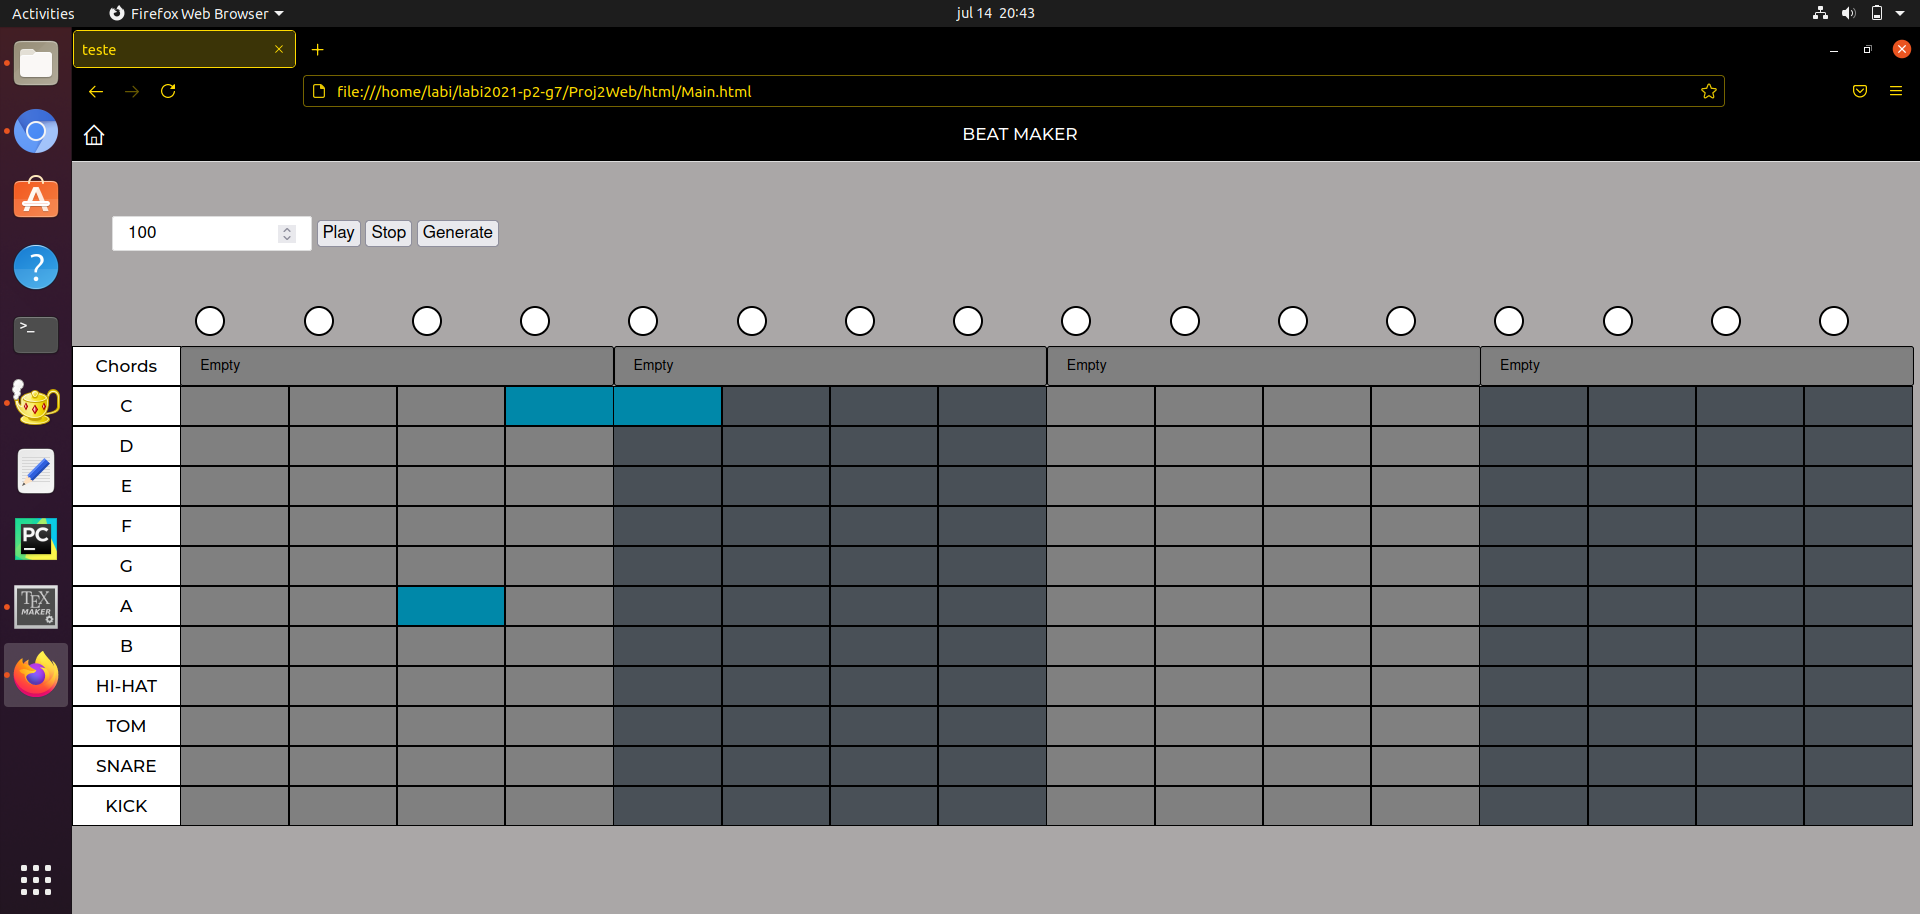
\includegraphics[width=7cm, height=4cm]{\beatmaker}
\label{Print do nosso beatmaker}
\end{figure}

\center Representação do beat maker do nosso trabalho. 
%
%%%%%%%%%%%%%%%%%%%%%%%%%%%%%%%%%%%%%%%%%%%%%%%%%%%%%%%%%
%%%%%CAPÍTULO 6: CONCLUSÃO
%
\chapter{Conclusão:}
\label{chap.conclusão}
\lhead{Conclusão}
A realização deste protejo deu-nos a oportunidade de aprofundar os nossos conhecimentos em phyton, pyaudio, cherrypy, data bases e um pouco mais em html. O projeto encontra-se no codeUa com o nome labi2021-p2-g7. 
\begin{figure}[h]
\center
\href{https://code.ua.pt//projects/labi2021-p2-g7}{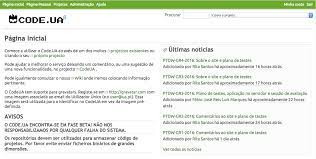
\includegraphics[width=7cm, height=4cm]{\codeua}}
\end{figure}
\center O link do nosso projeto, no code ua, pode ser acedido clicando na figura acima. 
%
%%%%%%%%%%%%%%%%%%%%%%%%%%%%%%%%%%%%%%%%%%%%%%%%%%%%%%%%%
%%%%%CONTRIBUIÇÕES DE AUTORES:
% 
\chapter*{Contribuições dos Autores}
\begin{table}[H]
    \centering
    \caption{Contribuições dos Autores.}
    \begin{tabular}{|c|c|c|c|c|}\hline
        Contribuição & Rui Machado & João Vieira & Inês Moreira & Pedro Cruzeiro  \\ 
        \hline
	    Produção de Relatório & 25~\% & 25~\% & 25~\% & 25~\%	\\
	    Aplicação Web & 25~\% & 25~\% & 25~\% & 25~\%	\\
	    Persistência & 25~\% & 25~\% & 25~\% & 25~\% \\
	    Gerador de Músicas & 25~\% & 25~\% & 25~\% & 25~\% \\
	    Gerador de Imagens & 25~\% & 25~\% & 25~\% & 25~\% \\ 
		Testes e Resultados & 25~\% & 25~\% & 25~\% & 25~\% \\
		   
    \hline
    \end{tabular}
    \label{tab.contribuições}
\end{table}	
%
%%%%%%%%%%%%%%%%%%%%%%%%%%%%%%%%%%%%%%%%%%%%%%%%%%%%%%%%%
%%%%%BIBLIOGRAFIA:
%
\begin{thebibliography}{9}
\bibitem{thinkpython} 
Allen Downey
\textit{Think Python - How to Think Like a Computer Scientist}. |
Green Tea Press, 2nd Edition, Version 2.4.0, 2015

\bibitem{stackoverflow} 
\textit{www.stackoverflow.com}. | acedido a 29/06/2021
\end{thebibliography}
\end{document}
